\scanpage{20}

à l'aide \unsure{en se donnant} un système

\diagram{\begin{tikzcd}[column sep=large]
\text{(35)} &
\begin{gathered}
\underline{\mathcal G}\supset\underline M\\[-2pt]
\text{Groupe sur }S_0,\\[-2pt]
\text{avec }\underline M\text{ comme}\\[-2pt]
\text{sous-groupe distingué}
\end{gathered}
& \text{, et }\Phi\colon\mathcal G_{S_0}\arrow[r]
& \underline{\mathcal G}
\end{tikzcd}}

tel que (34) se \unsure{reconstitue} à partir de (35) en prenant
$\underline M$, $\mathcal G_{S_0}$ dans (35),
$M_{S_0}$ \deleted{$\unsure{=}$} l'image inverse de
$\underline M\subset\underline{\mathcal G}$ par $\Phi$,
$\varphi$ induit par $\Phi$, et $\Theta$ l'opération déduite de
$\Phi$. De plus, $\Phi$ induit un \uline{iso}.

\diagram{\begin{tikzcd}
\underbrace{\mathcal G_{S_0}/M_{S_0}}_{H_{S_0}}
\arrow[r,"\sim"] & \underline{\mathcal G}/\underline M
\end{tikzcd}}

-- et on a là une description ``axiomatique'' du système (35)
en termes de (34).
La suite exacte de \deleted{\unsure{schémas}}\inserted{Groupes sur $S$}

\diagram{\begin{tikzcd}[column sep=large,row sep=small]
\text{(36)} & 1\arrow[r,dash] & \underline M\arrow[r]
& \underline{\mathcal G}\arrow[r]
& \underline{\mathcal G}/\underline M\arrow[r,dash]
\arrow[d,phantom,"\simeq"{description,rotate=90}] & 1\\
&&&& H_{S_0}.
\end{tikzcd}}

de fait, sur $\forall$ schém. de base affine $S$
(plus généralement, $S$ tel que $H^1(S,M\otimes_{\mathbb Z}\underline{\mathcal O}_S)=0$)
\unsure{des} suites exactes

\margin{L'hypothèse \unsure{faite} sur des $H^1$ \unsure{nul|nuls}
est entièrement inutile, car les $\underline M$-torseurs
\uline{sur} $S_0$ définis par les \unsure{images} \unsure{inverses}
des $h(\in H)$ sont \unsure{évidemment|d'ailleurs} triviaux}

\diagram{\begin{tikzcd}[column sep=large,row sep=small]
\text{(37)} & 1\arrow[r] & \underline M(S)\arrow[r]
\arrow[d,phantom,"\simeq"{description,rotate=90}]
& \underline{\mathcal G}\unsure{(A)|(/A)}\arrow[r]
& H_{S_0}(S)\arrow[r,dash]
\arrow[d,phantom,"\simeq"{description,rotate=90}] & 1\\
&& M\otimes_{\mathbb Z}A && H\text{ si }S\text{ conn.}\\[-3pt]
&&\text{si }S\text{ affine d'anneau }A
\end{tikzcd}}

\margin{19}

\scanpage{21}
\mspage{\unsure{658}}

En fait, on a par construction un \unsure{diagramme}
comm. de suites exactes

\diagram{\begin{tikzcd}[column sep=large,row sep=large]
\text{(38)} & 1\arrow[r] & M_{S_0}\arrow[r]\arrow[d]
&\mathcal G_{S_0}\arrow[r]\arrow[d]
&H_{S_0}\arrow[r,dash]
\arrow[d,phantom,"\unsure{\Downarrow}"{description}] &1\\
&1\arrow[r]&\underline M\arrow[r]
&\underline{\mathcal G}\arrow[r]&H_{S_0}\arrow[r]&1
\end{tikzcd}}

qui par passage aux sections donne \deleted{pour} $S$
\deleted{quelconque} affine (disons) connexe un diag. comm.

\diagram{\begin{tikzcd}[column sep=large,row sep=large]
\text{(39)} &1\arrow[r]&M\arrow[r]\arrow[d]
&\mathcal G\arrow[r]\arrow[d]
&H\arrow[r]\arrow[d,phantom,"\unsure{\Downarrow}"{description}]&1\\
&1\arrow[r]&M\otimes_{\mathbb Z}A\arrow[r]
&\underline{\mathcal G}(A)\arrow[r,dash]&H\arrow[r,dash]&1.
\end{tikzcd}}

Pour $S=S_0$ on retrouve l'iso (28) annoncé.

\margin{\uline{NB} En tant que faisceau (\unsure{sans} structure de
$S$-groupes) $\underline{\mathcal G}$ est isomorphe au
\deleted{\unsure{schéma}}\inserted{faisceau} somme des $H$ copies de
$\underline M$ -- il est donc représentable si $\underline M$ l'est.}

Cette construction du $\unsure{S_0}$-schéma en groupes
$\underline{\mathcal G}$, à partir d'une suite exacte (27), est
\unsure{manifestement} fonctorielle \unsure{p.r.|par.} à cette dernière :
un \unsure{hom.} de suites exactes

\diagram{\begin{tikzcd}[column sep=large,row sep=large]
\text{(40)}&1\arrow[r]&M\arrow[r]\arrow[d]
&\mathcal G\arrow[r]\arrow[d]&H\arrow[r]\arrow[d]&1\\
&1\arrow[r]&M'\arrow[r]&\mathcal G'\arrow[r]&H'\arrow[r,dash]&1
\end{tikzcd}}

donne naissance à un diag. comm. de suites exactes

\margin{20}

\scanpage{22}

\diagram{\begin{tikzcd}[column sep=small,row sep=large]
&1\arrow[rr,dash]&&M_{S_0}\arrow[rr]\arrow[dr]\arrow[dd]
&&\mathcal G_{S_0}\arrow[rr]\arrow[dr]\arrow[dd]
&&H_{S_0}\arrow[rr,dash]\arrow[dr]
\arrow[dd,dash,"\unsure{\Vert}"{description,pos=.25}]
&&1&\\
&&1\arrow[rr,"\deleted{\unsure{1}}"{description,pos=.15},crossing over]
&&M'_{S_0}\arrow[rr]\arrow[dd]
&&\mathcal G'_{S_0}\arrow[rr]\arrow[dd]
&&H'_{S_0}\arrow[rr]\arrow[dd]&&1\\
\text{(41)}&1\arrow[rr]&&\underline M^{\unsure{\cdot}}\arrow[rr]\arrow[dr]
&&\underline{\mathcal G}\arrow[rr]\arrow[dr]
&&H_{S_0}\arrow[rr]\arrow[dr]&&1&\deleted{\unsure{1}}\\
&&1\arrow[rr]&&\underline M'\arrow[rr]
&&\underline{\mathcal G}'\arrow[rr]
&&\underline H'\arrow[rr]&&1
\end{tikzcd}}

\margin{\uline{Enveloppe schématique} \uline{discrète}
\uline{des groupes} \uline{métabéliens}}

4. Reprenons donc un $\mathbb Z$-module libre de type fini $M$, et pour
$\forall$ sous-\deleted{\unsure{g}}\inserted{$\mathbb Z$}-module
d'indice fini, considérons la suite exacte

\diagram{\begin{tikzcd}[column sep=large]
\text{(42)}&1\arrow[r,dash]&M_i\arrow[r,dash]&M\arrow[r,dash]
&M/M_i\arrow[r,dash]&1.
\end{tikzcd}}

Plus \unsure{gén.}, si on part d'une suite exacte (27), pour
$\forall$ sous-groupe $M_i$ d'indice fini dans $M$,
\unsure{distingué} dans $\mathcal G$ i.e. stable par $H$,
on a une suite exacte

\diagram{\begin{tikzcd}[column sep=large]
\text{(43)}&1\arrow[r]&M_i\arrow[r]&\mathcal G\arrow[r]
&\underbrace{\mathcal G/M_i}_{H_i}\arrow[r,dash]&1
\end{tikzcd}}

où maintenant $H_i=\mathcal G/M_i$ \unsure{est} \unsure{une}
extension de

\diagram{\begin{tikzcd}[column sep=large]
\text{(44)}&1\arrow[r]&M/M_i\arrow[r]&H_i\arrow[r]&H\arrow[r]&1
\end{tikzcd}}

déduite de (27) par

\diagram{\begin{tikzcd}
M\arrow[r]&M/M_i.
\end{tikzcd}}

\margin{21}

\scanpage{23}
\mspage{\unsure{659}}

On note que \deleted{si $H$ est un groupe \unsure{ayant} un
\unsure{nb} fini de \unsure{gén.}, pour $H$ fini},
\deleted{alors} les $M_i\subset M$ d'indice fini et stables sous $H$
sont cofinaux dans l'\unsure{ens} de tous les $M_i$ d'indice fini dans
$M$. Considérons donc la suite exacte de sch. en groupes associée

\margin{prendre les $nM$ !}

\diagram{\begin{tikzcd}[column sep=large]
\text{(45)}&1\arrow[r]&\underline{M_i}\arrow[r]
&\underline{\mathcal G}_i\arrow[r]&H_{i\,S_0}\arrow[r]&1
\end{tikzcd}}

Pour $i$ variable, elles forment un syst. projectif d'extensions,
donc une extension de \unsure{progroupes} sur $S_0=\operatorname{Spec}\mathbb Z$.

\deleted{En particulier}

\deleted{\uline{\unsure{Remarque|Le pro-groupe}} $\unsure{\underline{\mathcal G}}$}

On considère le pro-objet $(\underline{\mathcal G}_i)$ comme pro-objet
de $C$ catégorie des schémas en groupes (lisses etc ...) sur $S_0$.
On note que les morphismes de transition

\diagram{\begin{tikzcd}
\underline{\mathcal G}_j\arrow[r]&\underline{\mathcal G}_i
\end{tikzcd}}

sont \uline{affines} -- la question étant locale
\inserted{sur $\underline{\mathcal G}_i$}, on est ramené à la voir pour
l'hom

\deleted{\unsure{image}}

\diagram{\begin{tikzcd}[column sep=large,row sep=small]
\unsure{E}(M_i,M_j)\arrow[r]
&E(M_i,M_i)\arrow[d,phantom,"\unsure{\Vert}"{description}]\\
M_i\supset M_j&\underline{M_i}\\[-3pt]
\text{ext. de }(M_i/M_j)_{S_0}\text{ par }\underline{M_j}
\end{tikzcd}}

\margin{22}

\scanpage{24}

Or le premier est affine, comme somme finie de schémas affines, le deuxième est affine --- donc le morphisme est affine.

Ceci étant, la limite projective des $\underline{\mathcal{G}}_i$ dans la catégorie des schémas existe (plus précisément, le foncteur limite projective des $\underline{\mathcal{G}}_i$ est représentable) --- il n'est peut être pas absurde de passer à la limite \unsure{carrément}, et de travailler avec ce schéma en groupes --- pas de t.f.

\uline{Remarque} Le pro-groupe $(\underline{\mathcal{G}}_i)$ sur $S_0=\operatorname{Spec}\unsure{\mathcal{G}|\mathbb{Z}}$ ne dépend que du \deleted{$\mathcal{G}$}, groupe discret $\mathcal{G}$, muni d'une classe de sous-groupes \inserted{\deleted{\unsure{invariants} abéliens}} modulo commensurabilité --- l'hypothèse à faire est que parmi ces sous-groupes, il y en a qui sont des $\mathbb{Z}$-modules \deleted{libres} de type fini (car les prenant assez petits, ils sont \uline{libres} de t.f.). Si $M_0$ est lui-même d'indice fini dans $\mathcal{G}$ i.e. si \deleted{les}\inserted{\unsure{un des|$\forall$ des}} $H_i$ sont finis,

\margin{23}

\scanpage{25}
\mspage{\unsure{660|680}}

alors ce proobjet ne dépend que de $\mathcal{G}$ lui
$\overline{\mathrm m}$ --- \unsure{soumis} à la condition qu'il existe
un sous-groupe d'indice fini dans $\mathcal{G}$ qui
soit un groupe commutatif, de t.f. en
tant que $\mathbb{Z}$-module. (On dit alors
que $\mathcal{G}$ est "\uline{métabélien}".)

\margin{\unsure{3}}
\deleted{Regardons le cas typique}

Ainsi, pour $\forall$ groupe discret
\inserted{$\mathcal{G}$} métabélien, on a construit un proschéma
en groupes, \inserted{syst. proj. de schémas en groupes \uline{affines},}
que je vais noter
\[
(46)\qquad
\operatorname{Env}(\mathcal{G})=(\underline{\mathcal{G}}_i)
\]
(l'ens d'indices étant formé des sous-groupes
distingués de $\mathcal{G}$ qui sont comm. et sans
torsion). Ce pro-groupe dépend \unsure{fonctoriellement}
de $\mathcal{G}$. Il a des propriétés \unsure{d'exactitudes|d'exactitude}
\unsure{intéressantes} et $\pm$ évidentes, p. ex.
il est multiplicatif
\[
(47)\qquad
\operatorname{Env}(\mathcal{G}\times\mathcal{G}')
\unsure{\xrightarrow{\sim}}
\operatorname{Env}(\mathcal{G})\mathbin{\times_{S_0}}
\operatorname{Env}(\mathcal{G}').
\]
Si on a une suite exacte
\[
(48)\qquad
\diagram{\begin{tikzcd}[column sep=large]
1 \arrow[r] & \mathcal{G}'' \arrow[r,no head] &
\mathcal{G} \arrow[r,no head] & \mathcal{G}' \arrow[r,no head] & 1
\end{tikzcd}}
\]
de groupes métabéliens, on a une suite
exacte pour les enveloppes
\[
(49)\qquad
\diagram{\begin{tikzcd}[column sep=large]
1 \arrow[r] & \underline{\operatorname{Env}}(\mathcal{G}'') \arrow[r] &
\operatorname{Env}(\mathcal{G}) \arrow[r,no head] &
\operatorname{Env}(\mathcal{G}') \arrow[r] & \unsure{1}
\end{tikzcd}}
\]

\margin{24}

\scanpage{26}

en un sens qu'il convient de préciser \unsure{à}
l'occasion --- pour les schémas en groupes
associés (obtenus en passant à la limite) ---
\unsure{on a bel et bien} un hom fid plat dont
le noyau est le bon \ldots

Le cas typique, auquel le cas général
se ramène de façon \unsure{assez} immédiate, est
celui où $\mathcal{G}=M=\mathbb{Z}$. On a pour
$\forall$ entier $n\geq 1$ la suite exacte
\[
(50)\qquad
\diagram{\begin{tikzcd}[column sep=large]
1 \arrow[r,no head] &
\mathbb{Z} \arrow[r,no head,"n"] &
\mathbb{Z} \arrow[r,no head] &
\mathbb{Z}/n\mathbb{Z} \arrow[r,no head] & 1
\end{tikzcd}}
\]
je vais \deleted{\unsure{construire}} expliciter la construction
de l'extension correspondante de
$\mathbb{Z}/n\mathbb{Z}$ par $\underline{\mathbb{Z}}=\mathbb{G}_a$,
soit $\underline{\mathcal{G}}_n$.

C'est un schéma affine, dont l'anneau
de coordonnées est isomorphe --- de façon pas
bien canonique --- au produit des
$n$ copies de celui de $\underline{\mathbb{Z}}=\mathbb{G}_a$,
savoir $\mathbb{Z}[T]$ --- on trouve un tel \unsure{isomorphisme}
en \unsure{choisissant} une section ensembliste de
$\mathbb{Z}$ sur $\mathbb{Z}/n\mathbb{Z}$, par exemple par \unsure{l'ens}
des entiers $\mathbb{Z}\cap[0,n-1]$. Les hom de

\margin{25}

\scanpage{27}
\mspage{\unsure{661|681}}

transition entre les $\underline{\mathcal{G}}_n$ n'ont rien de
plat bien sûr. Passant à la limite projective,
on trouve une extension de
\[
(\widehat{\mathbb{Z}})_{S_0}
\overset{\mathrm{dfn}}{=}
\varprojlim_n(\mathbb{Z}/n\mathbb{Z})_{S_0}
\]
--- schéma en groupes profini constant sur $S_0$ ---
par la limite projective des schémas
$\mathbb{G}_a$, s'envoyant dans lui $\overline{\mathrm m}$
par les hom
\unsure{vus} \deleted{\unsure{des} \unsure{\S b}} de $2^\circ$)
--- c'est le spectre
de l'anneau limite inductive des
\[
\begin{gathered}
\mathbb{Z}[T_n]\subset\mathbb{Q}[T]\\
T_n=\frac{1}{n}T
\end{gathered}
\]
qui est ainsi, chose étrange, \unsure{la}
\inserted{\unsure{sous-}}$\mathbb{Z}$-algèbre
de $\mathbb{Q}[T]$ \unsure{formé|formée} des polynômes
dont \uline{le terme constant} est un entier.

On a une \unsure{description} analogue de
la limite projective de l'enveloppe
schématique de $\mathbb{Z}^n$ --- c'est une
extension de $(\widehat{\mathbb{Z}}^{\,n})_{S_0}$
(attention à l'abus
de notation) par une composante neutre,
qui est le spectre du sous-anneau
de $\mathbb{Q}[T_1,\ldots,T_n]$ formé des polynômes dont
le terme constant est entier \ldots

\margin{26}

\scanpage{28}

C'est donc un schéma en groupes sur $S_0=\operatorname{Spec}\mathbb{Z}$
dont toutes les fibres sont réduites au groupe
unité, sauf la fibre \unsure{générique}, qui est
$ {\mathbb{G}_a^{\,n}}_{\mathbb{Q}}$.

\deleted{\unsure{Et}}
Dans le cas d'un groupe métabélien
quelconque $\mathcal{G}$, \unsure{désignant|désignons} par
$\widehat{\mathcal{G}}$ son
\unsure{complétifié} profini, par $\widehat{\mathcal{G}}_{S_0}$ le schéma
en groupes profini sur $\unsure{S_0}$.
\[
(50)\qquad
\widehat{\mathcal{G}}_{S_0}
\overset{\mathrm{dfn}}{=}\varprojlim_i(H_i)_{S_0}
\]
on \unsure{en} aura une suite exacte canonique
\[
(51)\qquad
\diagram{\begin{tikzcd}[column sep=large]
1 \arrow[r] &
\operatorname{Env}^{0}(\mathcal{G})
\arrow[r,very thick,"\deleted{\unsure{\mathrm{dfn}}}"] &
\varprojlim\operatorname{Env}(\mathcal{G}) \arrow[r] &
(\widehat{\mathcal{G}})_{S_0} \arrow[r] & 1
\end{tikzcd}}
\]
où $\operatorname{Env}^{0}(\mathcal{G})$ désigne la comp. neutre
de $\varprojlim\operatorname{Env}(\mathcal{G})$, i.e.
\[
\begin{aligned}
(52)\qquad
\operatorname{Env}^{0}(\mathcal{G})
&\overset{\mathrm{dfn}}{=}\varprojlim_i\underline{M}_i\\
&\simeq\varprojlim_n n.\,\underline{M}_0
\end{aligned}
\]
où les $M_i$ sont les sous-groupes d'indice
fini de $\mathcal{G}$ \deleted{\unsure{tels q|tel q}}
qui sont des $\mathbb{Z}$-modules libres de t.f., où
(comme plus haut) pour un tel $\mathbb{Z}$-module $M$,

\figure{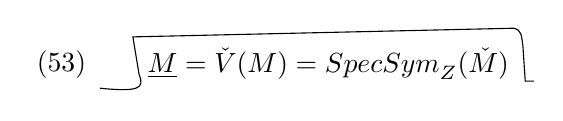
\begin{tikzpicture}[baseline=(eq.base)]
\node[anchor=base west,inner sep=0pt] (eq) at (0,0)
{$\underline{M}=\check{V}(M)=\operatorname{Spec}\operatorname{Sym}_{\mathbb{Z}}(\check{M})$};
\node[anchor=east] at ([xshift=-0.65cm]eq.west) {$(53)$};
\draw
([xshift=-0.60cm,yshift=-0.10cm]eq.south west)
.. controls ([xshift=-0.10cm,yshift=-0.15cm]eq.south west)
and ([xshift=-0.03cm,yshift=-0.10cm]eq.south west)
.. ([xshift=-0.10cm,yshift=0.07cm]eq.south west)
-- ([xshift=-0.18cm,yshift=0.14cm]eq.north west)
-- ([xshift=0.05cm,yshift=0.25cm]eq.north east)
.. controls ([xshift=0.16cm,yshift=0.23cm]eq.north east)
and ([xshift=0.15cm,yshift=0.15cm]eq.north east)
.. ([xshift=0.17cm,yshift=0.03cm]eq.north east)
-- ([xshift=0.20cm,yshift=-0.01cm]eq.south east)
-- ([xshift=0.31cm,yshift=-0.01cm]eq.south east);
\end{tikzpicture}}
désigne le fibré-vectoriel \unsure{cov.|can.} en $M$ qu'il définit, et

\margin{27}

\scanpage{29}
\mspage{\unsure{662|682}}

où $M_0$ est un des $M_i$, donnant lieu
au syst. (cofinal dans celui de tous les
$M_i$) des $nM_0$. Le choix d'une
base de $M_0$ sur $\mathbb{Z}$ donne un
iso
\[
(54)\qquad
\begin{aligned}
\operatorname{Env}^{0}(\mathcal{G})
&\simeq \operatorname{Env}^{0}(M_0)
\simeq \bigl(\operatorname{Env}^{0}(\mathbb{Z})^{\unsure{0}}\bigr)^n\\
&\simeq(\mathcal{E}^{1})^n
\end{aligned}
\]

\margin{$\unsure{\dagger}$ où
\diagram{\begin{tikzcd}[column sep=large]
(\mathbb{E}^{1},\unsure{mn|nm}) \arrow[r] &
(\mathbb{E}^{1},\uuline{n})
\end{tikzcd}}
est la multiplication par $m$}

\[
(55)\qquad
\begin{aligned}
\mathcal{E}^{1}
&\simeq \operatorname{Env}^{0}(\mathbb{Z})
\simeq\operatorname{Spec}\bigl(\mathbb{Z}+T\mathbb{Q}[T]\bigr)\\
&\inserted{\simeq\varprojlim_n(\mathbb{E}^{1},n)\,\unsure{\dagger}}
\end{aligned}
\]
est le schéma en groupes envisagé plus
haut, qui représente le foncteur en groupes
\[
(56)\qquad
A\longmapsto\mathcal{E}^{1}(A)
=\deleted{\unsure{\varprojlim}}
\left\{(x_n)\in A^{\mathbb{N}^{*}}\ \middle|\
\begin{gathered}
x_n=mx_{mn}\\[-2pt]
\forall m,n\in\unsure{\mathbb{N}^{*}}
\end{gathered}
\right\}.
\]

[Si $A$ est tel qu'il existe $n\in\mathbb{N}^{*}$ avec
$nA\,\unsure{\geq|\simeq}\,0$ ---
\deleted{\unsure{précis.}}
ce qui signifie
que les car. résiduelles de $A$ divisent $n$,
et \deleted{\unsure{c'est}} il existe sans doute un tel $n$
dès que les car. résiduelles de $A$ sont
toutes $>0$ --- alors $\mathcal{E}^{1}(A)=\{1\}$ ---
si par contre $A$ de car $0$, on a $\mathcal{E}^{1}(A)\simeq A$]

\margin{28}

\scanpage{30}

5. \uline{Caractérisation universelle} de l'enveloppe schématique d'un groupe métabélien.

Soit $G$ un schéma en groupes \unsure{loc.} de prés. finie sur une base $S$.
On dit qu'un \unsure{hom.} de schémas en groupes
\diagram{\begin{tikzcd}
H \arrow[r] & G
\end{tikzcd}}
est \deleted{\unsure{quasi-}} \uline{unipotent} (resp. quasi-unipotent) si l'image de $\forall$ \unsure{élt} de $H$ est un élément unipotent (resp. quasi unipotent) de $G$ --- ce qui se vérifie fibre par fibre. Un \unsure{hom.} d'un groupe discret
\diagram{\begin{tikzcd}
\mathcal{G} \arrow[r] & \Gamma(G/S)
\end{tikzcd}}
est dit unipotent (resp. quasi-unipotent) si l'\unsure{hom.} des schémas en groupes \deleted{\unsure{associé}} \inserted{qui lui correspond}
\diagram{\begin{tikzcd}
\mathcal{G}_S \arrow[r] & G
\end{tikzcd}}
est unipotent (resp. quasi-unipotent).

\margin{29}

\scanpage{31}
\mspage{\unsure{663|683}}

Notons que d'après les propriétés des $\varprojlim$ de syst. projectifs filtrants (à morphismes de transition affines) \deleted{entre} de schémas, si $\mathcal{G}$ est métabélien, d'où un système projectif de schémas en groupes affines sur $S_0$, donc sur $S$, noté $\operatorname{Env}_{\unsure{\underline{S}|S}}(\mathcal{G})$, et une limite projective
\[
\begin{aligned}
(57)\qquad L\operatorname{Env}_S(\mathcal{G})
 &=L\operatorname{Env}(\mathcal{G})\times_{S_0}S\\
 &\simeq\varprojlim\operatorname{Env}_S(\mathcal{G}),
\end{aligned}
\]
on a, dès que $G$ est \unsure{loc.} de prés. finie

(58)\quad
\diagram{\begin{tikzcd}[column sep=large,row sep=large]
\operatorname{Hom}_{\mathrm{progr}/S}(\operatorname{Env}_S(\mathcal{G}),G)
 \arrow[r,"\sim"] \arrow[d,equal,"\mathrm{def}"']
 & \operatorname{Hom}(\operatorname{Env}_S(\mathcal{G}),G)\\
\varprojlim_i\unsure{\operatorname{Hom}}(\underline{\mathcal{G}}_{i\,S},G) &
\end{tikzcd}}

Notons d'autre part qu'on a un \deleted{\unsure{un}} \unsure{hom.} canonique

(59)\quad
\diagram{\begin{tikzcd}
\mathcal{G}_S \arrow[r] & \deleted{\unsure{\varprojlim}}L\operatorname{Env}_S(\mathcal{G})
\end{tikzcd}}
déduit par \unsure{changement} de base de l'\unsure{hom.} sur la base universelle $S_0$

(59 bis)\quad
\diagram{\begin{tikzcd}
\mathcal{G}_{S_0} \arrow[r] & L\operatorname{Env}(\mathcal{G})
\end{tikzcd}}
provenant du système d'\unsure{hom.} can.

\margin{30}

\scanpage{32}

\diagram{\begin{tikzcd}
\underline{\mathcal{G}}_{S_0}\arrow[r]&\underline{\mathcal{G}}_i
\end{tikzcd}}.

Donc, via (59) on trouve

(60)\quad
\diagram{\begin{tikzcd}[column sep=large,row sep=large]
\operatorname{Hom}_{S\text{-}\mathrm{gr}}(L\operatorname{Env}_S(\mathcal{G}),G)
 \arrow[r] & \operatorname{Hom}_{S\text{-}\mathrm{gr}}(\mathcal{G}_S,G)
 \arrow[d,phantom,"\simeq"{rotate=90}]\\
 & \operatorname{Hom}_{\mathrm{gr}}(\mathcal{G},\Gamma(G/S))
\end{tikzcd}}

\unsure{1}

\unsure{Composant} (58) et (60), on trouve
\[
(61)\quad\left\{
\begin{aligned}
&\operatorname{Hom}_{\mathrm{pro}\text{-}S\text{-}\mathrm{gr}}\unsure{\ell}
 (\operatorname{Env}_S(\mathcal{G}),G)
 \simeq\operatorname{Hom}_{S\text{-}\mathrm{gr}}(L\operatorname{Env}_S(\mathcal{G}),G)\\[1.2em]
&\hspace{5em}\longrightarrow\operatorname{Hom}_{S\text{-}\mathrm{gr}}(\mathcal{G}_S,G)
 \simeq\operatorname{Hom}_{\mathrm{gr}}(\mathcal{G},G(S))
\end{aligned}\right.
\]
Ceci posé, on a le résultat suivant

\uline{Théorème} \deleted{\unsure{Si}} Sous les conditions précédentes

\margin{\figure{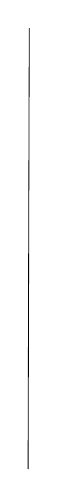
\begin{tikzpicture}
\draw[line width=.3pt] (0,0) -- (-.015,-5.6);
\end{tikzpicture}}}
($\mathcal{G}$ groupe discret métabélien, $G$ schéma en groupes loc. de prés. finie sur \unsure{schéma} de base $S$), l'application canonique (61) est \deleted{\uline{bijective} si on suppose de plus, pour ne pas \unsure{me|se} fatiguer, que} \inserted{injective, et a comme image} \unsure{l'ens.} des \unsure{hom.} \uline{quasi-unipotents} de $\mathcal{G}$ dans $G(S)$ --- du moins si on suppose, pour nous simplifier l'existence, que $S$ est \unsure{noeth.} et $G$ affine sur $S$.

\margin{31}

\scanpage{33}
\mspage{\unsure{664|684}}

\uline{\unsure{50}} \uline{Exemple} : La ``tour'' de Fermat.

1. Les groupes $\mathcal{G},\underline{\mathcal{G}}$.

Je m'intéresse au quotient de $\mathcal{G}_0^{\deleted{\unsure{\wedge}}}=\operatorname{GL}(2,\mathbb{Z})$ obtenu en prenant le quotient par $[\Pi_0,\Pi_0]$ --- on trouve une extension $\mathcal{G}$ de $\mathcal{G}_0/\Pi_0$ par le groupe

\margin{$\Pi_0$ engendré par les $\lambda_i=-\ell_i$,\quad
$\displaystyle \ell_0=\begin{pmatrix}1&-2\\0&1\end{pmatrix}$\quad
$\displaystyle \ell_1=\begin{pmatrix}1&0\\2&1\end{pmatrix}$.}

\[
\begin{aligned}
(1)\qquad M\overset{\mathrm{dfn}}{=}\Pi_{0\,\mathrm{ab}}
\simeq
\Bigl(
\underset{\deleted{\underbrace{\hphantom{\mathbb{Z}(0)+\mathbb{Z}(1)+\mathbb{Z}(\infty)}}_{M}}}
{\overset{\deleted{\unsure{\wedge}}}{\mathbb{Z}}(0)+
 \overset{\deleted{\unsure{\wedge}}}{\mathbb{Z}}(1)+
 \overset{\deleted{\unsure{\wedge}}}{\mathbb{Z}}(\infty)}
\Bigr)/\text{diagonale}
\end{aligned}
\]
Ainsi on a une suite exacte de groupes profinis

(2)\quad
\diagram{\begin{tikzcd}[column sep=large,row sep=large]
1\arrow[r] & M\arrow[r]\arrow[d,phantom,"\simeq"{rotate=90}]
 &\mathcal{G}\arrow[r]
 &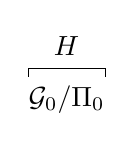
\begin{tikzpicture}[baseline=(q33.base)]
\node[inner sep=0pt] (q33) {$\mathcal{G}_0/\Pi_0$};
\draw[line width=.3pt] ([yshift=3pt]q33.north west)--([yshift=6pt]q33.north west)--([yshift=6pt]q33.north east)--([yshift=3pt]q33.north east);
\node[above=7pt] at (q33.north) {$H$};
\end{tikzpicture}\arrow[r]\arrow[d,phantom,"\simeq"{rotate=90}]
 &1\\
 &\begin{gathered}\Pi_{0\,\mathrm{ab}},\text{ noté aussi}\\\mathcal{G}^{\circ}\end{gathered}
 &&\operatorname{GL}(2,\mathbb{Z}/4\mathbb{Z})/(\dot{\ell}_0,\dot{\ell}_1)&
\end{tikzcd}}

Par générateurs et relations on a
\[
(3)\quad\mathcal{G}=\left\{\tau',\rho,\sigma\;\middle|\;
\begin{aligned}
&\rho^6=\sigma^4={\tau'}^2=1\\
&\rho^3=\sigma^2,\quad\tau'(\rho)=\rho^{-1},\quad\tau'(\sigma)=\sigma^{-1}\\
&\deleted{\unsure{\rho}}[\lambda_0,\lambda_1]=1,\quad\text{où}
\end{aligned}\right.
\]
\[
\hspace{8em}\left\{
\begin{aligned}
\lambda_0&=-\ell_0=-\sigma\rho\sigma\rho=\sigma(\rho)\rho^{\deleted{\unsure{-1|4}}}\\
\lambda_1&=-\ell_1=-\rho\sigma\rho\sigma=\rho\sigma(\rho)
\end{aligned}\right.
\]
\unsure{dont|donc} la relation de commutation $[\lambda_0,\lambda_1]=1$ s'écrit aussi
\[
(4)\qquad \sigma(\rho)\rho^2\sigma(\rho)=\rho\sigma(\rho^2)\rho
\qquad\text{ou encore}
\]
\[
(5)\qquad -\sigma\underbrace{\rho\sigma\rho^{-1}\sigma\rho}\sigma
=\underbrace{\rho\sigma\rho^{-1}\sigma\rho}
\]
où le jeu des signes $-$ peut s'expliciter dans le formalisme des gén. et rel. en supprimant dans la formule ce signe, et en remplaçant en \unsure{revanche} un (ou un \unsure{n\textsuperscript{b}|nb} impair) des $\sigma$ de la formule par des $\sigma^{-1}$. Par exemple, la formule

\margin{32}

\scanpage{34}

s'écrit, en introduisant

\margin{\uline{NB} $\lambda_\infty\overset{\mathrm{dfn}}{=}-\ell_\infty$}

\[
(6)\qquad
\lambda_\infty\deleted{\unsure{=-\ell_\infty}}
=\rho\sigma\rho^{-1}\sigma\rho
=\rho(\sigma)\sigma\rho
=-\rho\sigma(\rho)^{-1}\rho
=\rho\sigma\rho^{-1}(\sigma)
\]
sous la forme
\[
(7)\qquad [\sigma,\lambda_\infty]=1.
\]
\margin{NB $\sigma=\sigma_\infty$}

\margin{\uline{NB} On trouve
\[
\left\{
\begin{aligned}
[\ell_0,\ell_1]&=[\lambda_0,\lambda_1]=(\sigma(\rho)\rho^{-1})^3\\
[\underbrace{\sigma_{\deleted{\unsure{\infty}}}}_{\sigma}\unsure{,}\ell_\infty]
&=[\underbrace{\sigma_\infty}_{\sigma},\lambda_\infty]
=(\sigma(\rho^{-1})\rho)^3\\
&=\operatorname{int}(\sigma\rho^{-1})\cdot[\ell_0,\ell_1]
\end{aligned}\right.
\]}

On va définir un schéma en groupes \inserted{$\underline{\mathcal{G}}$} sur $\mathbb{Z}$, dont les \inserted{$\unsure{\widehat{\mathbb{Z}}|\mathbb{Z}}$-}pts seront \inserted{(à un \unsure{isom.|disons} près)} les pts de $\widehat{\mathcal{G}}$. On pose
\[
(8)\qquad
\underline{M}=\underline{\mathcal{G}}^{\circ}
=\unsure{\mathbb{G}_a|\mathbb{E}_a}^{\{0,1,\infty\}}/\text{diagonale}
\]
\margin{Il vaut mieux le \unsure{noter} $\underline{M}$ --- il y a déjà trop de $\mathcal{G}$ !}

On va faire opérer \deleted{$\unsure{\mathcal{G}/M}$}
\[
\deleted{(\unsure{4})}(4)\qquad
\mathcal{G}\deleted{\unsure{=\operatorname{GL}(2,\mathbb{Z})}}
\simeq\operatorname{GL}(2,\mathbb{Z})/[\Pi_0,\Pi_0]
\]
sur $\underline{M}\deleted{\unsure{=\underline{\mathcal{G}}^{\circ}}}$,
\deleted{\unsure{en décrivant ainsi}} \inserted{à travers}
\[
(5)\qquad
\underbrace{\mathcal{G}_3\times\mu_{\unsure{\tau|2}}^{\deleted{\unsure{2}}}}_{\simeq\unsure{\Gamma_{0,3}}}
\simeq\mathcal{G}/M\deleted{\unsure{\widehat{\mathbb{Z}}}}
\simeq\mathcal{G}_{0,3}/\Pi.
\]

Désignant par $\unsure{\overbrace{\dot{\lambda}_0,\dot{\lambda}_1}},\dot{\lambda}_\infty$ les images des
$\deleted{\lambda_0,\lambda_1}\lambda_i=-\ell_i$ dans $\deleted{\unsure{M}}\mathcal{G}$, identifiées à des éléments de
\[
M=\mathcal{G}^{\circ}=\underline{\mathcal{G}}^{\circ}(\widehat{\mathbb{Z}})
\]
--- en fait on a
\[
(6)\qquad
\left\{
\begin{aligned}
\dot{\lambda}_0\unsure{,|>}\dot{\lambda}_1,\dot{\lambda}_\infty
&\in\deleted{\unsure{\underline{\mathcal{G}}^{\circ}}}\inserted{\underline{M}}(\mathbb{Z})
\subset\deleted{\unsure{\underline{\mathcal{G}}^{\circ}}}\inserted{\underline{M}}(\widehat{\mathbb{Z}})
=M\otimes_{\unsure{\cdot|\mathbb{Z}}}\unsure{\mathbb{Z}|\widehat{\mathbb{Z}}}\\
\text{donc,}\quad\dot{\lambda}_0+\dot{\lambda}_1+\dot{\lambda}_\infty&=0
\end{aligned}\right.
\]
\margin{(ici on note additivement la loi de groupe dans $M=\underline{\mathcal{G}}^{\circ}$)}

\margin{\figure{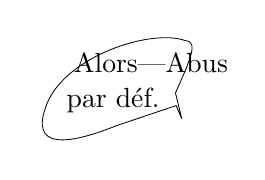
\begin{tikzpicture}[scale=.8]
\draw[line width=.3pt] (1.2,.85) .. controls (.65,1.05) and (-.7,.6) .. (-1,-.15)
 .. controls (-1.3,-.9) and (-.65,-.8) .. (.1,-.5)
 -- (1.05,-.18) -- (1.14,-.39) -- (1.04,.02)
 .. controls (1.25,.5) and (1.42,.84) .. (1.2,.85);
\node at (.65,.5) {\unsure{Alors|Abus}};
\node at (.05,-.1) {par déf.};
\end{tikzpicture}}}
$\mathcal{G}_3$ opère sur $\underline{M}=\underline{\mathcal{G}}^{\circ}$ par son action sur les \deleted{\unsure{bases}} \inserted{gén.} canoniques $\deleted{\unsure{\lambda_0}}\dot{\lambda}_0,\dot{\lambda}_1,\dot{\lambda}_\infty$, donc
\[
(7)\qquad
\left\{
\begin{aligned}
\sigma(\dot{\lambda}_0)&=\dot{\lambda}_1,\quad
\sigma(\dot{\lambda}_1)=\dot{\lambda}_0
\quad\inserted{\text{d'où}}\quad
\sigma(\dot{\lambda}_\infty)=\dot{\lambda}_\infty\\
\rho(\dot{\lambda}_i)&=\dot{\lambda}_{i+1}
\end{aligned}\right.
\]
\margin{Ceci se voit d'abord pour $i=0,1$ et, \unsure{s'en déduit} pour $i=\infty$.}
D'autre part on a par définition
\[
(8)\qquad\tau(\dot{\lambda}_i)=-\dot{\lambda}_i
\]
où
\diagram{\begin{tikzcd}[column sep=2pt,row sep=small]
\tau\arrow[d,equal]&{}={}&\sigma&\tau'\arrow[d,equal]\\
\tau_\infty&&&\tau'_\infty
\end{tikzcd}}

\margin{33}

\scanpage{35}
\mspage{\unsure{665|685}}

. L'extension $\underline{\mathcal G}$ annoncée est bien sûr celle de § 50 3°), \unsure{développé} entre-temps (depuis les premières lignes du présent §, constatant justement que j'étais gêné aux entournures pour expliciter la construction) :

(9)\quad\diagram{\begin{tikzcd}[column sep=large]
1 \arrow[r] & \underline M \arrow[r] \arrow[d,equal] & \underline{\mathcal G} \arrow[r] & H_{S_0} \arrow[r,no head] & 1 \\
 & \check V(M) & & &
\end{tikzcd}}
où $S_0=\operatorname{Spec}\mathbb Z$.

Pour $\unsure{\forall}$ schéma $S$, on posera
\[
\tag{10}
\begin{gathered}
\underline{\mathcal G}^{\Delta}(S)\subset\underline{\mathcal G}(S)\\
\Vert\;\mathrm{dfn}\\
\text{Image inverse de la ``diagonale'' de}\\
\Gamma(H_{\unsure{S|S_0}}/S)
\quad\bigl(\text{i.e. de l'image de }H\longrightarrow\Gamma(H_{\unsure{S|S_0}},S)\bigr)\\
\text{par l'hom. canonique }\underline{\unsure{\mathcal G|\mathcal E}}(S)\longrightarrow H_S(S),
\end{gathered}
\]
de sorte que par la construction du loc. cit. on aura un iso. canonique
\[
\tag{11}
\underline{\mathcal G}^{\Delta}(S)\simeq
\mathcal G\underset{M}{\wedge}\deleted{\unsure{A}}
\underbrace{\Gamma(S,\underline{\mathcal O}_S\otimes_{\mathbb Z}M)}_{
\simeq\deleted{\unsure{A}}\inserted{M}\otimes_{\mathbb Z}A\ \text{si}}
\]
et une suite exacte can.

(12)\quad\diagram{\begin{tikzcd}[column sep=large]
1 \arrow[r] & \underbrace{\Gamma(S,\underline{\mathcal O}_S\otimes_{\mathbb Z}M)}_{A\otimes_{\mathbb Z}M} \arrow[r] & \underline{\mathcal G}^{\Delta}(S) \arrow[r] & H \arrow[r] & 1.
\end{tikzcd}}

\figure{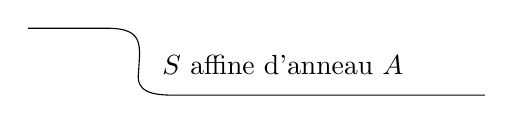
\begin{tikzpicture}[x=1cm,y=1cm]
\draw (0,0.75) -- (1.0,0.75)
.. controls (1.48,0.75) and (1.42,0.53) .. (1.40,0.18)
.. controls (1.37,-0.06) and (1.57,-0.10) .. (1.85,-0.10)
-- (5.80,-0.10);
\node[anchor=west] at (1.58,0.28) {$S$ affine d'anneau $A$};
\end{tikzpicture}}

Prenant $A=\widehat{\mathbb Z}$, on trouve en particulier (et c'est encore un fait général sur les schémas en groupes associés à des extensions de groupes discrets à noyau abélien)
\[
\tag{13}
\mathcal G^{\wedge}\simeq\underline{\mathcal G}^{\Delta}(\widehat{\mathbb Z}).
\]
\margin{34}

\scanpage{36}

2. Le groupe $\widetilde Z_{\rho,\sigma}$ : \uline{version provisoire}.

. Je vais maintenant expliciter pour $\widehat{\mathcal G}$ et $\widehat{\mathcal G}_{\unsure{0|\bullet}}\longrightarrow\widehat{\mathcal G}$ les constructions générales de § 49 $\overline{\underline{\mathrm{VI}}}$, en \inserted{y} prenant \deleted{$\unsure{\mathcal G}$}
\[
\tag{14}
\underline{\mathcal G}^{\unsure{\natural}}\overset{\mathrm{dfn}}=
\underline M=\underline{\mathcal G}^{\circ}
\quad(\text{composante neutre de }\underline{\mathcal G})
\]
Dans un cas comme celui-ci, où $\underline{\mathcal G}^{\unsure{\natural}}$ est justement le sous-groupe fermé du $(\rho,\sigma)$-groupe $\mathcal G_{\rho,\sigma}$ $(=\mathcal G^{\wedge}\text{ ici})$ engendré par $\lambda_0,\lambda_1,\lambda_\infty$, on se \unsure{dispensera} dans les notations --- là où il n'y a pas ambiguïté --- d'inclure la notation $\unsure{\natural}$. Pour \unsure{$\forall$ $A$} il y aura lieu de distinguer p.ex. entre $G_{\rho,\sigma}$ et $G_{\rho,\sigma}^{\unsure{\natural}}$ etc. \uline{Nous ferons cependant les constructions dans le cadre schématique, plutôt que profini.}

\margin{Je pense à la fin comparer les deux constructions possibles. Les \unsure{soulignés} indiqueront les \uline{schémas} en groupes...}

Le pas essentiel est de déterminer le groupe $\underline Z_{\rho,\sigma}$
\[
\tag{15}
\begin{gathered}
\underline Z_{\rho,\sigma}\subset\underline{\operatorname{Aut}}(\underline{\mathcal G}^{+})\\
\Vert\;\mathrm{dfn}\\
\left\{u\in\underline{\operatorname{Aut}}(\mathcal G^{+})\ \left|\
\begin{aligned}
\deleted{\unsure{1^{\circ}}}\ \text{a)}\;&\exists\alpha\in\underline{\mathcal G}_{\tau}^{\unsure{\natural}}=\{1,\tau\}.\underline M,
&&u(\rho)=\alpha(\rho)\\
\text{b)}\;&\exists\beta\in\text{-- -- -- -- -- --}
&&u(\sigma)=\beta(\sigma)\\
\text{c)}\;&u(L_0^{\deleted{\unsure{\Pi_0}}\mathcal G})=L_0^{\mathcal G}
&&\deleted{\unsure{(\Longleftrightarrow L_0^{\Pi_0}=L_0^{\natural})}}\\
&\qquad(\Longleftrightarrow u(L_0^{\Pi_0})=L_0^{\Pi_0})\\
\bigl[\text{d)}\;&(\text{automatique})\quad u(\mathcal G^{\unsure{\natural}})\subset\mathcal G^{\unsure{\natural}}\bigr]
\end{aligned}\right.\right.
\end{gathered}
\]

\margin{ici, ``$\exists\alpha$'' ``$\exists\beta$'' signifie bien sûr l'existence \uline{locale} de $\alpha,\beta$...}

Notons que $u$ est déterminé par les valeurs
\[
\tag{16}
\begin{cases}
u(\rho)=\xi\rho\\
u(\sigma)=\eta\sigma
\end{cases}
\qquad\xi,\eta\in\Gamma\underline\Pi
\]
\margin{où $\underline\Pi=\underline M\unsure{\rtimes}\deleted{\unsure{\{1,\tau\}}}\inserted{\unsure{\mu_2}}$ ($\underline M$ est gr. d'indice $2$ dans $\underline\Pi$)}
\inserted{$\xi,\eta$} satisfaisant les conditions suivantes ;
\margin{35}

\scanpage{37}
\mspage{\unsure{666|686}}

\[
\tag{17}
\left\{
\begin{aligned}
\text{a)}\;&\xi\rho\ \text{(localement) conjugué à }\rho\ \text{via }\underline{\unsure{\mathcal G}}^{\unsure{\natural}}=\underline M\\
\text{b)}\;&\eta\sigma\ \text{-- -- -- -- -- -- ---}\ \sigma\ \text{'' -- -- ---}\\
\text{c)}\;&\text{équation des lacets}\\
&\xi=\eta\ell_1^{\nu}\quad\text{où }\nu\in\Gamma\mathbb G_a\ \text{convenable}\\
&\qquad\bigl(\text{tel que }\mu\overset{\mathrm{dfn}}=2\nu+1\in\Gamma\mathbb G_m\bigr)
\end{aligned}\right.
\]

. \deleted{Comme $\xi,\eta\in\Gamma N$, il faudra}

\uline{Remarque} Il n'est plus possible ici de désigner par $-1$ l'élément non trivial \inserted{$\omega$} du centre $\unsure{\mu|\mu_2}$ de $\mathcal G^{\wedge}$, et de désigner par $-x$ (pour $x\in\mathcal G^{\wedge}$) le produit de $x$ par celui-ci, à cause de la confusion avec la notation $-x$ \inserted{(pour $x\in M$)} dans le groupe abélien $M$ pour l'inverse de $x$ --- mais \deleted{\unsure{l'élém.}} $\omega x\ne-x$, puisque $\omega x\notin M$, $-x\in M$...

On pose bien sûr
\[
\tag{18}
\varepsilon_3(u)=\varepsilon_{\mathcal G}(\alpha),\qquad
\varepsilon_2(u)=\varepsilon_{\mathcal G}(\beta)
\]
(bien défini, car $\rho$ et $\rho^{-1}$ ne sont conjugués sur aucune fibre, idem pour $\sigma,\sigma^{-1}$), comment les expliciter en termes de $\xi,\eta$ ? On aura

\deleted{\unsure{(17)}}
\[
\tag{19}
\left\{
\begin{aligned}
\xi=\alpha\rho(\alpha)^{-1}
&\left\{
\begin{aligned}
&\in\Gamma\underline M\quad\text{si }\alpha\in\Gamma\underline M=\Gamma\underline{\mathcal G}^{\unsure{\natural}}\ \text{i.e. }\varepsilon_3(u)=1\\
&=\underbrace{\alpha_0}_{\in\Gamma\underline M}\tau\rho(\alpha_0\tau)^{-1}
=\alpha_0\underbrace{(-\ell_1^{-1})}_{\lambda_1^{-1}\in\underline M}\rho(\alpha_0)^{-1}\in\Gamma\underline M\quad\text{si }\varepsilon_3(u)=\unsure{-1}
\end{aligned}\right.\\[1ex]
\eta=\beta\sigma(\beta)^{-1}
&\left\{
\begin{aligned}
&\in\Gamma\underline M\quad\text{si }\beta\in\Gamma\underline M=\Gamma\underline{\mathcal G}^{\unsure{\natural}}\ \text{i.e. }\varepsilon_2(u)=1\\
&=(\underbrace{\beta_0}_{\in\Gamma\underline M}\tau)\sigma(\beta_0\tau)^{-1}
=\omega\beta_0\sigma(\beta_0)^{-1}\in\omega\underline M\quad\text{si }\varepsilon_2(u)=\unsure{-1}
\end{aligned}\right.
\end{aligned}\right.
\]
donc en tous cas
\[
\tag{19 bis}
\begin{cases}
\xi\in\Gamma\underline M\\
\eta\in\Gamma\bigl(\omega^{\nu_2(u)}.\underline{\unsure{M|M'}}\bigr)
\end{cases}
\]
\margin{36}

\scanpage{38}
\mspage{676}

d'où on tire, par l'équation des lacets (17)
\[
\tag{20}
\ell_1^{\nu}=(\omega\lambda_1)^{\nu}\in\Gamma(\omega^{\nu_2(u)}.\underline M)
\quad\text{i.e. }\unsure{\Longleftrightarrow}\ \omega^{\nu}\in\Gamma(\omega^{\nu_2(u)}.\underline M)
\]
On peut l'écrire sous la forme
\[
\tag{21}
\underline\nu=2\underline\nu'+\underline\nu_2
\]
où
\[
\tag{22}
\left\{
\begin{aligned}
\underline\nu,\underline\nu' &: Z_{\rho,\sigma}\longrightarrow\mathbb G_a\\
\underline\nu_2,\underline\nu_3 &: Z_{\rho,\sigma}\rightrightarrows
(\mathbb Z/2\mathbb Z)_{S_0}^{\unsure{\mathrm{que}|\mathrm{cste}}}
\end{aligned}\right.
\]
\deleted{$\unsure{\varepsilon}$}
sont des \unsure{morphismes} de schémas bien définis, liés \inserted{entre eux et} aux hom. de groupes \deleted{$\unsure{\mu}$}
\[
\underline\mu:Z_{\rho,\sigma}\longrightarrow\mathbb G_m,\qquad
\underline\varepsilon_{\unsure{1|2}},\underline\varepsilon_3:Z_{\rho,\sigma}\longrightarrow\{\pm1\}_{S_0}
\]
par les formules (21) et
\[
\tag{23}
\left\{
\begin{aligned}
\underline\mu&=2\underline\nu\,\unsure{+}\,1\deleted{\unsure{+1}}
\quad(=4\underline\nu'\,\unsure{+}\,2\underline\nu_2+1)\\
\underline\varepsilon_2&=(-1)^{\underline\nu_2},\qquad
\underline\varepsilon_3=(-1)^{\underline\nu_3}.
\end{aligned}\right.
\]

On aura donc, en vertu de (\unsure{24|21})
\deleted{
\[
\tag{24}
\ell_1^{\nu}=\ell_1^{2\nu'}\ell_1^{\nu_2}
=\underbrace{(\omega\lambda_1)}_{\lambda_1}^{2\nu'}\ell_1^{\nu_2}
=\lambda_1^{2\nu'}\ell_1^{\nu_2}
\]
Comme $\ell_1=\lambda_1\omega$, on
\deleted{j'ai envie de mettre les $\ell_i$ sous la forme}
\[
\tag{25}
\ell_i=a_i\omega\quad\text{où }a_i\in\underline M!
\]
peut \deleted{\unsure{pour ainsi|pourra}} écrire (24) sous la forme
\[
\tag{26}
\ell_1^{\nu}=\underbrace{(\lambda_1^{\unsure{2\nu'}}a_1^{\nu_2})}_{\in\Gamma\underline M}\omega^{\nu_2}
\quad\deleted{\text{pour }\unsure{\nu_2=0|\nu_2=1}\ \text{i.e. }\unsure{\varepsilon_2=1}}
\]
Pour expliciter les $a_i$, il faut les développer en combinaisons linéaires de $\lambda_0,\lambda_1,\lambda_\infty$ (ou de deux d'entre eux, si on veut unicité).
}
\margin{37}
